% Author: Izaak Neutelings (November 2020)
\documentclass[border=3pt,tikz]{standalone}
\usepackage{physics}
\usepackage{tikz}
\usepackage[outline]{contour} % glow around text
\usetikzlibrary{patterns,decorations.pathmorphing}
\usetikzlibrary{decorations.markings}
\usetikzlibrary{arrows.meta}
\usetikzlibrary{calc}
\tikzset{>=latex}
\contourlength{1.1pt}

\colorlet{mydarkblue}{blue!40!black}
\colorlet{myblue}{blue!70!black}
\colorlet{myred}{red!65!black}
\colorlet{myorange}{orange!90!black!90}
\colorlet{vcol}{green!45!black}
\colorlet{watercol}{blue!80!cyan!10!white}
\colorlet{darkwatercol}{blue!80!cyan!80!black!30!white}
\colorlet{metalcol}{blue!25!black!30!white}
\tikzstyle{piston}=[blue!50!black,top color=blue!30,bottom color=blue!50,middle color=blue!20,shading angle=0]
\tikzstyle{water}=[draw=mydarkblue,rounded corners=0.1,top color=watercol!90,bottom color=watercol!90!black,middle color=watercol!50,shading angle=20]
\tikzstyle{horizontal water}=[water,top color=watercol!90!black!90,bottom color=watercol!90!black!90,middle color=watercol!80,shading angle=0]
\tikzstyle{metal}=[draw=metalcol!10!black,rounded corners=0.1,top color=metalcol,bottom color=metalcol!80!black,shading angle=10]
\tikzstyle{vvec}=[->,very thick,vcol,line cap=round]
\tikzstyle{force}=[->,myred,very thick,line cap=round]
\tikzstyle{width}=[{Latex[length=4,width=3]}-{Latex[length=4,width=3]}]
\def\tick#1#2{\draw[thick] (#1)++(#2:0.12) --++ (#2-180:0.24)}

\begin{document}



% LAMINAR FLOW around object
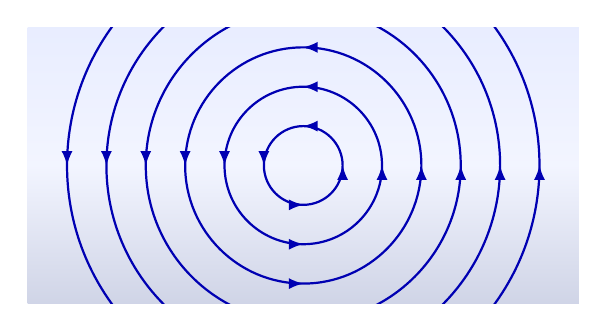
\begin{tikzpicture}
  \def\W{7.0}   % total length
  \def\H{3.5}   % total height
  \def\R{1.0}   % total distance
  \def\N{5}     % number of layers
  \def\t{\H/\N} % layer thickness
  % \draw[water,shading angle=0,draw=none]
    % (-0.52*\W,-0.52*\H) rectangle (0.52*\W,0.52*\H);
  % \draw[metal]
    % (0,0) circle(\R);

      % Clip to desired aspect ratio
  \clip (-0.5*\W,-0.5*\H) rectangle (0.5*\W,0.5*\H);
  
    \draw[water,shading angle=0,draw=none]
    (-0.52*\W,-0.52*\H) rectangle (0.52*\W,0.52*\H);
    
  % draw exact field lines for a vortex flow : radial lines are circles
  % use foreach over radius 
  \foreach \r in {0.5,1,...,3} {
    \draw[myblue,thick,postaction={decorate},decoration={markings,
        mark=at position {0} with {\arrow{latex}},mark=at position {0.25} with {\arrow{latex}},mark=at position 0.5 with {\arrow{latex}}, mark=at position 0.75 with {\arrow{latex}}}] (0:\r) arc (0:360:\r);
  }
 
\end{tikzpicture}



\end{document}
